% das Papierformat zuerst
\documentclass[a4paper, 11pt]{article}
% deutsche Silbentrennung
\usepackage[ngerman]{babel}
% wegen deutschen Umlauten
\usepackage[utf8]{inputenc}
% andere pdfs einbinden
\usepackage{pdfpages}
% um bilder einzubinden
\usepackage{graphicx}
% fuer source code listings
\usepackage{listings}
% seitenränder
\usepackage[left=3cm,right=3cm,top=2cm,bottom=2cm]{geometry}
% um hyperlinks einfügen zu können
\usepackage{hyperref}
% um weitere Symbole zu nutzen
\usepackage{amssymb}
% um weitere Operatoren zu nutzen
\usepackage{amsmath}
%Aufzaehlung
\usepackage{paralist}
%Beachtet, ob ein Leerzeichen syntaktisch passt oder nicht
\usepackage{xspace}
% um hyperlinks einfügen zu können
\usepackage{hyperref}
%um Kopf- und Fußzeile zu bearbeiten
\usepackage{fancyhdr}
%um Literaturverzeichnis auch im Inhaltsverzeichnis anzuzeigen
\usepackage{tocbibind}
%um Silbentrennungen angeben zu können, welche nicht unterstützt werden
\RequirePackage[ngerman=ngerman-x-latest]{hyphsubst}
%um Tabellen zu begrenzen, damit sie nicht in den Rand hineinragen
\usepackage{tabularx}
%um die landscape Umgebung zu nutzen (Querformat)
\usepackage{pdflscape}

%ermöglicht Anführungsstriche unten und oben
\newcommand{\su}{\glqq} %unten
\newcommand{\so}{\grqq\xspace} %oben mit anschließendem Leerzeichen
\newcommand{\soo}{\grqq} %nur oben

%ermöglicht eckige Klammern
\newcommand{\eka}{$<$} %<
\newcommand{\ekz}{$>$\xspace} %> mit anschließendem Leerzeichen

%Versionsnummer
\newcommand{\version}{0.0}

% Tabellenabschnitt linksbündig
\newcommand{\ltab}{\raggedright\arraybackslash}
% Tabellenabschnitt zentriert
\newcommand{\ctab}{\centering\arraybackslash}
% Tabellenabschnitt rechtsbündig
\newcommand{\rtab}{\raggedleft\arraybackslash}

%Einstellungen für Fuß- und Kopfzeile
\pagestyle{fancy}
\fancyhf{}
\fancyhead[L]{\footnotesize M. Lüdemann $\cdot$ M. Butkereit $\cdot$ W. Schumacher $\cdot$ A. Melkonyan $\cdot$ M. Colbow $\cdot$ M. Cakir\\ Requirements and Design Documentation $\cdot$ ESEP WS2016(v\version) $\cdot$ HAW Hamburg}
%\fancyhead[C]{\footnotesize}
\fancyhead[R]{\footnotesize \today}
%\renewcommand{\headrulewidth}{0.0pt}
\fancyfoot[C]{\thepage}

%Stil des Literaturverzeichnisses bestimmen
\bibliographystyle{unsrt}

\begin{document}

% Den Titel festlegen
\title
{
    Requirements and Design Documentation\\
    \bigskip
    (RDD)\\
    \medskip
    {\normalsize Version \version}\\
    \bigskip
    ESEP - Praktikum - Wintersemester 2016
}

% Autor/en
\author
{
\begin{tabular}{llll}
Lüdemann&Mona&2212744&mona.luedemann1@haw-hamburg.de\\
Butkereit&Marvin&2247550&marvin.butkereit@haw-hamburg.de\\
Schumacher&Wilhelm&2245216&wilhelm.schumacher@haw-hamburg.de\\
Melkonyan&Anushavan&2243668&anushavan.melkonyan@haw-hamburg.de\\
Colbow&Marco&2177095&marco.colbow@haw-hamburg.de\\
Cakir&Mehmet&2195657&mehmet.cakir@haw-hamburg.de
\end{tabular}
}

% Erstelle die Titelseite
\maketitle

\noindent {\large Änderungshistorie:}
\begin{table}[h]
\begin{tabularx}{\textwidth}{|c|c|c|X|}
\hline
\textbf{Version} & \textbf{Author} & \textbf{Datum} & \centering\arraybackslash \textbf{Anmerkungen/Änderungen}\\
\hline
 &  &  &  \\
\hline
\end{tabularx}
\label{changes}
\end{table}

\newpage

\tableofcontents

\newpage

\section{Teamorganisation}
Grundsätzlich kann jedes Teammitglied eine Aufgabe seiner Wahl übernehmen. Die Aufgaben, dessen Verteilung bei jedem Meeting neu beschlossen wird, richten sich nach den zu bewältigenden Milestones(siehe \cite{esep}) zum jeweiligen Praktikumstermin. Allerdings wurden für die Projektleitung und die Pflege des RDD-Dokuments jeweils eine Person bestimmt, welche im Unterkapitel \ref{vantw} eingesehen werden können.

\subsection{Verantwortlichkeiten}\label{vantw}
\begin{table}[h]
\center
\begin{tabularx}{\textwidth}{|l|l|X|}
\hline
\textbf{Aufgabe}&\textbf{Zuständige/r}&\textbf{Bemerkung}\\
\hline
Projektleitung&Mona&Die Projektleitung hält den Fortschritt im Auge und benachrichtigt insbesondere bei Nichteinhalten des Zeitplans alle Teammitglieder. Außerdem hat die Projektleitung bei Unstimmigkeiten immer das letzte Wort. \\
\hline
RDD-Pflege&Mehmet&Der Zuständige ist für die Gestaltung und für die Vollständigkeit des RDDs verantwortlich. Er kann andere Gruppenteilnehmer dazu auffordern Inhalte für das Dokument zu erarbeiten und ihm bereit zu stellen. \\
\hline 
Protkollführung&Alle Teammitglieder&Die Protokollführung wird reihum von einem anderen Gruppenmitglied übernommen. Dabei wird folgende Reihenfolge eingehalten: $Mona\rightarrow Marvin\rightarrow Marco \rightarrow Wilhelm\rightarrow Mehmet\rightarrow Anushavan$ \\
\hline
\end{tabularx}
\caption{Zuteilung von Verantwortlichkeiten}
\label{labelname}
\end{table}

\subsection{Absprachen}
Zur Kommunikation außerhalb der Praktikumstermine werden Slack und WhatsApp verwendet. Unstimmigkeiten, Fragen und Inkenntnissetzung können somit interaktiv geklärt bzw. mitgeteilt werden. Es wird erwartet, dass jedes Teammitglied so schnell wie möglich darauf reagiert. In folgender Abbildung \ref{meets} werden die Termine der Meetings dargestellt:
\begin{figure}[h]
\centering 
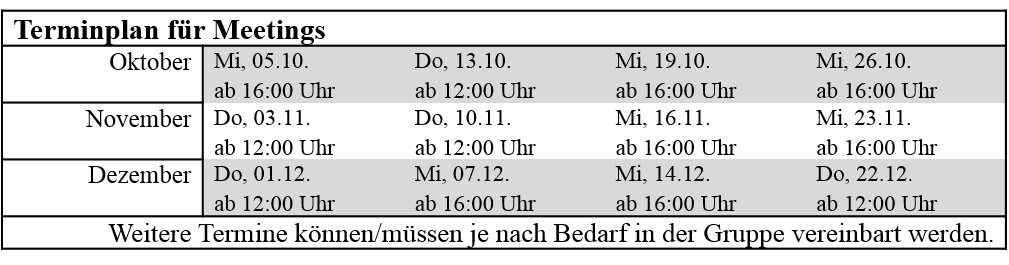
\includegraphics[scale=0.85]{images/Terminplan_Meetings.png}
\caption{Terminplan der Meetings}
\label{meets}
\end{figure}

\newpage

\subsection{Repository-Konzept}
Das Projekt wird mit dem Versionskontrollsystem Git verwaltet. Zentral wurde ein Repository auf GitHub angelegt. Erreichbar ist das Repository unter \url{https://github.com/mbutkereit/conveyor}. Änderungen werden lokal auf einem anderen Branch als auf dem Master vorgenommen. Wenn die Änderungen gepusht werden sollen, muss zuvor auf den Master Branch gewechselt und gepullt werden. Nun kann ein Merge mit dem lokal anderen Branch durchgeführt und ggf. Mergekonflikte gelöst werden. Anschließend kann gepusht werden.

\section{Projektmanagement}
Für die Gewährleistung eines guten Managements, werden in den folgenden Kapiteln erklärt wie die Teammitglieder mit ihren Aufgaben umgehen bzw. wann eine gegenseitige Benachrichtigung über ihren Fortschritt spätestens stattfinden sollte.

\subsection{Prozess}
Das Projekt wird auf Grundlage der geforderten Milestones nach und nach umgesetzt. Für jede Implementierung ist zuvor ein geeignetes sowie größtenteils selbsterklärendes bzw. verständliches, aber auch möglichst vollständiges Diagramm anzufertigen. Bestenfalls sollte die Visualisierung vor der Implementierung allen anderen Teammitgliedern vorgestellt werden, um mögliche Verbesserungen einzuholen und ggf. Konflikte früh zu erkennen sowie sie zu lösen.

\subsection{PSP/Zeitplan/Tracking}
Zu jedem Praktikumstermin wird erwartet, dass die verteilten Aufgaben bzw. Milestones erfüllt werden. Um dies möglichst zu gewährleisten, muss jedes Teammitglied bei Schwierigkeiten andere Teammitglieder darüber sofort in Kenntnis setzen, damit frühzeitig ausgeholfen werden kann.

\subsection{Qualitätssicherung}
Hinsichtlich der Qualitätssicherung, werden die vier Punkte Team, Modellierung, Code und Förderband herangezogen.
\medskip
\begin{compactenum}[1.]
\item \textbf{Team:} Jedes Teammitglied sollte über seine eigenen Fähigkeiten im Klaren sein und möglichst nur Aufgaben übernehmen, wofür es sich am besten geeignet fühlt. Darüber hinaus muss jedes Teammitglied bei Möglichkeit stets seine Unterstützung anbieten. Bei Problemen oder Überforderung müssen alle anderen Teammitglieder darüber unterrichtet werden und Aufgaben ggf. neu verteilt werden.
\medskip
\item \textbf{Modellierung:} Vor der Implementierung muss eine geeignete Visualisierung erstellt, anderen Teammitgliedern vorgestellt und untereinander diskutiert werden. 
\medskip
\item \textbf{Code:} Der Code wird nach beschlossenen Konventionen gefertigt. Dabei werden bekannte Pattern eingesetzt und möglichst einfache sowie übersichtliche Realisierungen angestrebt.
\medskip
\item \textbf{Förderband:} Um hohen Durchsatz sowie Effizienz bei der Aussortierung zu erzielen, werden die Komponenten mit der höchstmöglichen Leistung für die jeweilige Situation angetrieben, während die Sicherheit des Bedieners im Vordergrund steht. Dabei werden Fehler- bzw. Ausnahmezustände ggf. durch einfache Signalcodes mithilfe der Ampel dem Bediener mitgeteilt.
\end{compactenum}

\section{Randbedingungen}
In diesem Kapitel werden die Bedingungen genannt unter denen das Projekt umgesetzt wird und die Mittel, die für die Umsetzung herangezogen werden.

\subsection{Entwicklungsumgebung}
Die beiden Förderbänder werden über zwei QNX Systeme gesteuert, die über eine serielle Schnittstelle verbunden sind. Als IDE wird QNX Momentics auf Windows 7 verwendet.

\subsection{Werkzeuge}
\begin{compactenum}[-]
\item QNX Momentics IDE 5.0
\item Latex
\item Git(GitHub)
\end{compactenum}

\subsection{Sprachen}
Das System wird in C++ 11 programmiert. Die dazukommenden Bibliotheken sind in folgender Tabelle \ref{bibl} aufgelistet:
\medskip
\begin{table}[h]
\center
\begin{tabular}{|l|l|l|}
\hline
\textbf{Name}&\textbf{Version}&\textbf{Autor}\\
\hline
HWaccess.h&Unknown&Prof. Dr. Stephan Pareigis\\
\hline
HAWThread.h&Unknown&Prof. Dr. Stephan Pareigis \\
\hline
Lock.h&0.1&Simon Brummer \\
\hline
\end{tabular}
\caption{Verwendete Programmierbibliotheken}
\label{bibl}
\end{table}

\newpage

\section{Requirements and Use Cases}

\subsection{Systemebene}
\subsubsection{Stakeholder}
\begin{table}[h]
\center
\begin{tabularx}{\textwidth}{|X|X|}
\hline
\textbf{Stakeholder}&\textbf{Interessen}\\
\hline
Kunde&\begin{compactenum}[-]
      \item fehlerfreie Umsetzung der Anforderungen
      \item erfolgreiche Beendigung des Projektes 
      \end{compactenum}\\
\hline
Designer&\begin{compactenum}[-]
         \item übersichtliches, leicht erweiterbares Design
         \item sorgfältige Dokumentation 
         \end{compactenum}\\ 
\hline
Entwickler&\begin{compactenum}[-]
           \item präzises Design
           \item sinnvolle Kommentare
           \item lesbarer Code 
           \end{compactenum}\\
\hline
Tester&\begin{compactenum}[-]
       \item übersichtliches, vollständiges Testkonzept 
       \end{compactenum}\\
\hline
Bediener (Mitarbeiter, die das Laufband später bedienen sollen)&\begin{compactenum}[-]
\item einfache und intuitive Bedienung
\end{compactenum}\\
\hline
Instanthalter&\begin{compactenum}[-]
              \item robustes System
              \end{compactenum}\\
\hline
Andere Mitarbeiter&\begin{compactenum}[-]
                   \item Kenntnis über System und Funktionsweise
                   \end{compactenum}\\
\hline
\end{tabularx}
\caption{Stakeholder und ihre Interessen}
\label{stake}
\end{table}

\newpage

\subsubsection{Anforderungen}
\begin{table}[h]
\center
\begin{tabularx}{\textwidth}{|X|X|}
\hline
\textbf{Titel}&\textbf{Beschreibung}\\
\hline
Ansteuerung der Ampel&Das System soll die Ampel ansteuern können:
\begin{compactenum}[-]
\item grünes Licht bei Normalbetrieb, fehlerfrei 
\item gelbes Licht bei Warnings 
\item rotes Licht bei Errors 
\end{compactenum}\\
\hline
Ansteuerung der Motoren der Laufbänder&Die Motoren der Laufbänder sollen ansteuerbar sein in folgenden Varianten: 
\begin{compactenum}[-]
\item Rechtslauf 
\item Linkslauf 
\item Langsam 
\item Stopp
\end{compactenum}\\
\hline
Ansteuerung der Weiche&Eine prinzipielle Ansteuerung der Weichen soll möglich sein. Außerdem soll beachtet werde, dass die Weichen nur für kurze Zeit auf Durchgang gestellt werden dürfen, um eine Beschädigung des System zu vermeiden.\\
\hline
Erkennung von Werkstücken&Das System muss drei Arten von Werkstücke zuordnen können: 
\begin{compactenum}[-]
\item Flache Werkstücke 
\item Werkstücke mit Metalleinsatz (Bohrung liegt nach oben oder unten) 
\item Werkstücke ohne Metalleinsatz (Bohrung liegt nach oben oder unten)
\end{compactenum}\\
\hline
Aussortierung von Werkstücken&Flache Werkstücke und Werkstücke, bei der die Bohrung nach unten liegt, sollen aussortiert werden. \\
\hline
Reihenfolge der Werkstücke&Am Ende von Band 2 sollen die Werkstücke vereinzelt ankommen in der Reihenfolge:\hspace{2cm}
$Bohrung oben ohne Metall\rightarrow Bohrung oben ohne Metall\rightarrow Bohrung oben mit Metall$ \\
\hline
\end{tabularx}
\caption{Anforderungen(Teil 1)}
\label{anf1}
\end{table}

\newpage

\begin{table}[h]
\center
\begin{tabularx}{\textwidth}{|X|X|}
\hline
\textbf{Titel}&\textbf{Beschreibung}\\
\hline
Erkennung von Überschlagen der Werkstücke + Aussortierung des betreffenden Werkstücks&Das System soll erkennen, wenn sich Werkstücke bei der Übergabe von Band 1 zu Band 2 überschlägt und das betreffende Werkstück soll anschließend auf Band 2 aussortiert werden.\\
\hline
Langsamer Transport bei Höhenmessung&Wenn ein Werkstück durch die Höhenmessung transportiert wird, soll das Förderband langsam laufen.\\
\hline
Konsolenausgabe am Ende von Band 2&Wenn ein Werkstück das Ende von Band 2 erreicht, sollen auf der Konsole folgende Werkstückdaten ausgegeben werden:
\begin{compactenum}[-]
\item ID 
\item Typ 
\item Höhen-Messwert von Band 1 
\item Höhen-Messwert von Band 2 
\end{compactenum}\\
\hline
Konsolenausgabe am Ende von Band 3&Am Ende des dritten Bandes sollen die Werkstückdaten aller drei Werkstücke ausgegeben werden.\\
\hline
Stopp der Bänder bei keinen Werkstücken&Alle drei Bänder sollen jeweils stoppen, wenn sich kein Werkstück auf ihnen befindet.\\
\hline
Erkennung voller Rutschen&Volle Rutschen müssen erkannt werden.\\
\hline
Rutschen koordinieren&Ist die Rutsche auf Band 1 voll, so soll die Aussortierung über Band 2 erfolgen. Umgekehrt, ist die Rutsche auf Band 2 voll, so soll die Aussortierung bereits auf Band 1 erfolgen.\\
\hline
Gebündelter Transport von Werkstückgruppen auf Band 3&Die drei sortierten Werkstücke sollen gebündelt (im Abstand von 0-2cm) an das Ende des dritten Bandes transportiert werden. Der Platz zwischen den Dreiergruppen soll möglichst gering sein.\\
\hline
Fehlererfassung: Verschwinden von Werkstücken + Reaktion&Es soll erkannt werden, wenn Werkstücke verschwinden mittels der zu langen Laufzeit zwischen den Lichtschranken. Reaktion: Bandstopp, Fehlermeldung\\
\hline
\end{tabularx}
\caption{Anforderungen(Teil 2)}
\label{anf2}
\end{table}

\newpage

\begin{table}[h]
\center
\begin{tabularx}{\textwidth}{|X|X|}
\hline
\textbf{Titel}&\textbf{Beschreibung}\\
\hline
Fehlererfassung: Hinzufügen von Werkstücken + Reaktion&Er soll erkannt werden, wenn Werkstücke hinzugefügt werden mittels der zu kurzen Laufzeit zwischen den Lichtschranken. Reaktion: Bandstopp, Fehlermeldung \\
\hline
Fehlererfassung: Beide Rutschen voll + Reaktion&Es soll erkannt werden, wenn beide Rutschen voll sind. Reaktion: Bandstopp, Fehlermeldung \\
\hline
\end{tabularx}
\caption{Anforderungen(Teil 3)}
\label{anf3}
\end{table}

\subsubsection{Systemkontext}
\textbf{Port A (Ausgabeport)}
\begin{table}[h]
\center
\begin{tabularx}{\textwidth}{|X|X|}
\hline
\textbf{Ereignis}&\textbf{Methodenname}\\
\hline
Motor Rechtslauf&\begin{compactenum}[]
           \item \ttfamily right()
           \end{compactenum}\\
\hline
Motor Linkslauf&\begin{compactenum}[]
           \item \ttfamily fast()
           \end{compactenum}\\
\hline
Motor Langsam&\begin{compactenum}[]
           \item \ttfamily stop()
           \end{compactenum}\\
\hline
Motor Stopp&\begin{compactenum}[]
           \item \ttfamily stop()
           \end{compactenum}\\
\hline
Weiche Auf&\begin{compactenum}[]
           \item \ttfamily switchOpen()
           \item \ttfamily switchClosed()
           \end{compactenum}\\
\hline
Ampel Grün&\begin{compactenum}[]
           \item \ttfamily turnGreenOn()
           \item \ttfamily turnGrennOff()
           \end{compactenum}\\
\hline
Ampel Gelb&\begin{compactenum}[]
           \item \ttfamily turnYellowOn()
           \item \ttfamily turnYellowOff()
           \end{compactenum}\\
\hline
Ampel Rot&\begin{compactenum}[]
           \item \ttfamily turnRedOn()
           \item \ttfamily turnRedOff()
           \end{compactenum}\\
\hline
\end{tabularx}
\caption{API auf Port A(Ausgabeport)}
\label{portA}
\end{table}

\newpage

\noindent\textbf{Port B (Eingabeport)}
\begin{table}[h]
\center
\begin{tabularx}{\textwidth}{|X|X|}
\hline
\textbf{Ereignis}&\textbf{Methodenname}\\
\hline
Einlauf Werkstück&\begin{compactenum}[]
           \item \ttfamily isItemRunningIn()
           \end{compactenum}\\
\hline
Werkstück in Höhenmessung&\begin{compactenum}[]
           \item \ttfamily isItemAltimetry()
           \end{compactenum}\\
\hline
Höhenmessung&\begin{compactenum}[]
           \item \ttfamily isItemInAltimetryToleranceRange()
           \end{compactenum}\\
\hline
Werkstück in Weiche&\begin{compactenum}[]
           \item \ttfamily isItemSwitch()
           \end{compactenum}\\
\hline
Werkstück Metall&\begin{compactenum}[]
           \item \ttfamily isItemMetal()
           \end{compactenum}\\
\hline
Weiche offen&\begin{compactenum}[]
           \item \ttfamily isSwitchOpen()
           \end{compactenum}\\
\hline
Rutsche voll&\begin{compactenum}[]
           \item \ttfamily isSkidFull()
           \end{compactenum}\\
\hline
Auslauf Werkstück&\begin{compactenum}[]
           \item \ttfamily isItemRunningOut()
           \end{compactenum}\\
\hline
\end{tabularx}
\caption{API auf Port B (Eingabeport)}
\label{portB}
\end{table}

\newpage

\noindent\textbf{Port C (Ein-/Ausgabeport)}
\begin{table}[h]
\center
\begin{tabularx}{\textwidth}{|X|X|}
\hline
\textbf{Ereignis}&\textbf{Methodenname}\\
\hline
LED Starttaste&\begin{compactenum}[]
           \item \ttfamily turnLedStartOn()
           \item \ttfamily turnLedStartOff()
           \end{compactenum}\\
\hline
LED Resettaste&\begin{compactenum}[]
           \item \ttfamily turnLedResetOn()
           \item \ttfamily turnLedResetOff()
           \end{compactenum}\\
\hline
LED Q1&\begin{compactenum}[]
           \item \ttfamily turnLedQ1On()
           \item \ttfamily turnLedQ1Off()
           \end{compactenum}\\
\hline
LED Q2&\begin{compactenum}[]
           \item \ttfamily turnLedQ2On()
           \item \ttfamily turnLedQ2Off()
           \end{compactenum}\\
\hline
Taste Start&\begin{compactenum}[]
           \item \ttfamily isButtonStartPressed()
           \end{compactenum}\\
\hline
Taste Stopp&\begin{compactenum}[]
           \item \ttfamily isButtonStopPressed()
           \end{compactenum}\\
\hline
Taste Reset&\begin{compactenum}[]
           \item \ttfamily isButtonResetPressed()
           \end{compactenum}\\
\hline
Taste E-Stopp&\begin{compactenum}[]
           \item \ttfamily isButtonEStopPressed()
           \end{compactenum}\\
\hline
\end{tabularx}
\caption{API auf Port C (Ein-/Ausgabeport)}
\label{portC}
\end{table}

\newpage

\subsubsection{Use Cases}

\begin{compactenum}[1.]
\item Flache Werkstücke aussortieren
\medskip

\textbf{Akteure:} Mitarbeiter (legt die Werkstücke auf das Band), Höhenmessung, Weiche
\medskip

\textbf{Auslösendes Ereignis:} Höhenmessung erkennt das flache Werkstück.
\medskip

\textbf{Kurzbeschreibung:} Die flachen Werkstücke werden auf Band 1 mit der Höhenmessung erkannt und über die Weiche aussortiert.
\bigskip

\item Werkstückdaten ausgeben
\medskip

\textbf{Akteure:} Lichtschranke, Display
\medskip

\textbf{Auslösendes Ereignis:} Die Lichtschranke auf Band 2 wird durchquert.
\medskip

\textbf{Kurzbeschreibung:} Wenn ein Werkstück das Ende von Band 2 erreicht, werden die Werkstückdaten auf dem Display ausgegeben.
\bigskip

\item Ausgabe der Werkstücke auf Band 3 in der richtigen Reihenfolge
\medskip

\textbf{Akteure:} Lichtschranke, Mitarbeiter (nimmt die Werkstücke im Empfang), Weiche
\medskip

\textbf{Auslösendes Ereignis:} Es sind die drei richtigen Werkstücke auf Band 3 vorhanden.
\medskip

\textbf{Kurzbeschreibung:} Auf Band 3 werden jeweils 3 Werkstücke gebündelt in der richtigen Reihenfolge ($Bohrung oben ohne Metall\rightarrow Bohrung oben ohne Metall\rightarrow Bohrung oben mit Metall$) ausgegeben.
\end{compactenum}

\subsection{Systemanalyse}
\textcolor{red}{Ihr technisches System hat aus Sicht der Software bestimmte Eigenschaften. Was muss man für die Entwicklung der Software in Struktur, Schnittstellen, Verhalten und an Besonderheiten wissen? Wählen sie eine Kapitelstruktur, die am besten zur Dokumentation ihrer Ergebnisse geeignet ist.}

\subsection{Softwareebene}
\textcolor{red}{Sie sollen Software für die Steuerung des technischen Systems erstellen. Aus den Anforderungen auf der Systemebene und der Systemanalyse ergeben sich Anforderungen für Ihre Software. Insbesondere wird sich die Software der beiden Anlagenteile in einigen Punkten unterscheiden. Dokumentieren sie hier die Anforderungen, die sich speziell für die Software ergeben haben.}

\subsubsection{Systemkontext}
\textcolor{red}{Wie sieht der Kontext Ihrer Software aus? Wie erfolgt die Kommunikation mit Nachbarsystemen? Liste der ein- und ausgehenden Signale/Nachrichten.}

\subsubsection{Anforderungen}
\textcolor{red}{Welche wesentlichen Anforderungen ergeben sich aus den Systemanforderungen für ihre Software? Achten sie auf die entsprechende Attribuierung. Berücksichtigen sie auch mögliche Fehlbedienungen und Fehlverhalten des Systems.}

\section{Design}
\textcolor{red}{Anmerkung: Die Implementierung MUSS zu Ihrem Design-Modell konsistent sein. Strukturen, Verhalten und Bezeichner im Code müssen mit dem Modell übereinstimmen. Daher ist ein wohlüberlegtes Design wichtig.}

\subsection{System Architektur}
\textcolor{red}{Erstellung sie eine Architektur für Ihre Software. Geben sie eine kurze Beschreibung Ihrer Architektur mit den dazugehörenden Komponenten und Schnittstellen an. Dokumentieren sie hier wichtige technische Entscheidungen. Welche Pattern werden gegebenenfalls verwendet? Wie erfolgt die interne Kommunikation?}

\subsection{Datenmodellierung}
\textcolor{red}{Bestimmen sie das Datenmodell und dokumentieren sie es hier mit Hilfe von UML Klassendiagrammen unter Beachtung der Designprinzipien. Die Modelle können mit Hilfe eines UML-Tools erstellt werden. Hier ist dann ein Übersichtsbild einzufügen.
Geben sie eine kurze textuelle Beschreibung des Datenmodells und deren wichtigsten Klassen und Methoden an.
}

\subsection{Verhaltensmodellierung}
\textcolor{red}{Ihre Software muss zur Bearbeitung der Aufgaben ein Verhalten aufweisen. Überlegen sie sich dieses Verhalten auf Basis der Anforderungen und modellieren sie das Verhalten unter Verwendung von Verhaltensdiagrammen. Sie können für die Spezifikation der Prozess-Lenkung entweder Petri-Netze oder hierarchische Automaten verwenden. Die Modelle können mit Hilfe eines UML-Tools erstellt werden. Hier sind dann kommentierte Übersichtsbilder einzufügen.}

\section{Implementierung}
\textcolor{red}{Anmerkung: Nur wichtige Implementierungsdetails sollen hier erklärt werden. Code-Beispiele (snippets) können hier aufgelistet werden, um der Erklärung zu dienen. 
Anmerkung: Bitte KEINE ganze Programme hierhin kopieren!
}

\section{Testen}
\textcolor{red}{Machen sie sich auf Basis ihrer Überlegungen zur Qualitätssicherung Gedanken darüber, wie sie die Erfüllung der Anforderungen möglichst automatisiert im Rahmen von Unit-Test, Komponententest, Integrationstest, Systemtest, Regressionstest und Abnahmetest überprüfen werden.}

\subsection{Testplan}
\textcolor{red}{Definieren sie Zeitpunkte für die jeweiligen Teststufen in ihrer Projektplanung. Dazu können sie die Meilensteine zu Hilfe nehmen.}

\subsection{Testkonzept}
\begin{table}[h]
\center
\begin{tabularx}{\textwidth}{|X|X|X|}
\hline
\textbf{Funktion:}&\textbf{Test erfolgreich}&\textbf{Anmerkung}\\
\hline
Erkennung der Werkstücke am Anfang des Förderbandes&&\\
\hline
Flache Werkstücke werden aussortiert&&\\
\hline
Bei der Aussortierung der flachen Werkstücke blinkt die gelbe Leuchte&&\\
\hline
Werkstücke mit der Bohrung nach unten werden aussortiert&&\\
\hline
Bei Förderband 1, Fehlermeldung bei voller Rutsche&&\\
\hline
Bei Förderband 2, Fehlermeldung und Stopp von Förderband 1 und Förderband 2 bei voller Rutsche&&\\
\hline
Stopp beim leeren Förderband&&\\
\hline
Beim Verschwinden von Werkstücken wird eine Fehlermeldung ausgegeben und das Förderband stoppt&&\\
\hline
Beim Hinzufügen von Werkstücken mitten auf dem Förderband wird eine Fehlermeldung ausgegeben und das Förderband stoppt&&\\
\hline
Am Ende von Band 2 soll die gewünschte Reihenfolge der Werkstücke entstehen&&\\
\hline
Am Ende vom Band 2 werden die Werkstückdaten ausgegeben auf der Konsole&&\\
\hline
\end{tabularx}
\caption{Testauswertung(Teil 1)}
\label{tst1}
\end{table}

\newpage

\begin{table}[h]
\center
\begin{tabularx}{\textwidth}{|X|X|X|}
\hline
\textbf{Funktion:}&\textbf{Test erfolgreich}&\textbf{Anmerkung}\\
\hline
Am Ende vom Band 3 werden die Werkstückdaten als 3er Gruppe ausgegeben auf der Konsole&&\\
\hline
Förderband 3 transportiert die Werkstücke erst dann bis zum Ende des Bandes wenn die 3er Gruppe vollständig ist.&&\\
\hline
\end{tabularx}
\caption{Testauswertung(Teil 2)}
\label{tst2}
\end{table}

\subsection{Abnahmetest}
\textcolor{red}{Leiten sie die Abnahmebedingungen aus den Kunden-Anforderungen her. Dokumentieren sie hier, welche Schritte für die Abnahme erforderlich sind und welches Ergebnis jeweils erwartet wird (Test Cases).}

\subsection{Testprotokolle und Auswertungen}
\textcolor{red}{Hier fügen sie die Test Protokolle bei, auch wenn Fehler bereits beseitigt worden sind, ist es schön zu wissen, welche Fehler einst aufgetaucht sind. Eventuelle Anmerkung zur Fehlerbehandlung kann für weitere Entwicklungen hilfreich sein.
Das letzte Testprotokoll ist das Abnahmeprotokoll, das bei der abschließenden Vorführung erstellt wird. Es enthält eine Auflistung der erfolgreich vorgeführten Funktionen des Systems sowie eine Mängelliste mit Erklärungen der Ursachen der Fehlfunktionen und Vorschlägen zur Abhilfe
}

\section{Lessons Learned}
\textcolor{red}{Führen sie ein Teammeeting durch in dem gesammelt wird, was gut gelaufen war, was schlecht gelaufen war und was man im nächsten Projekt (z.B. im PO) besser machen will. Listen sie für die Aspekte jeweils mindestens drei Punkte auf. Weitere Erfahrungen und Erkenntnisse können hier ebenso kommentiert werden, auch Anregungen für die Weiterentwicklung des Praktikums.}

\section{Anhang}

\subsection{Glossar}
\textcolor{red}{Eindeutige Begriffserklärungen}

\subsection{Abkürzungen}
\textcolor{red}{Listen sie alle Abkürzungen auf, die sie in diesem Dokument benutzt haben.}

\end{document}

% Weitere Syntax für verschiedene Anwendungsfelder

%Aufzählungen
%\begin{compactenum}[1.]
%\item
%\end{compactenum}

%\ref{labelname des zu Referenzierenden Objekts}

%Tabelle
%\begin{table}[h]
%\center
%\begin{tabular}{|l|l|}
%\hline
%\textbf{linke Spaltenüberschrift}&\textbf{rechte Spaltenüberschrift}\\
%\hline
%1&2\\
%\hline
%3&4\\
%\end{tabular}
%\caption{Zugriffsoperationen}
%\label{labelname}
%\end{table}

%Tabelle mit tabularx
%\begin{table}[h]
%\center
%\begin{tabularx}{\textwidth}{|l|X|}
%\hline
%Text in linker Spalte&Text in rechter Spalte der über den Rand hinausragt\\
%\hline
%\end{tabularx}
%\caption{Tabellenunterschrift}
%\label{labelname}
%\end{table}

%Grafik einfügen
%\begin{figure}[h]
%\centering 
%\includegraphics[scale=0.3]{Dateiname}
%\caption{Bildunterschrift}
%\label{labelname}
%\end{figure}

%Linksbündig mit definierter Einrückung
%\begin{flushleft}
%\leftskip0.6cm
%\end{flushleft}

%Codelisting
%\lstset{basicstyle=\ttfamily}
%\begin{lstlisting}
%Code
%\end{lstlisting}

%Erzeugen eines Inhaltsverzeichnisses und ihrer Einträge
%\tableofcontents
%\section{•}
%\subsection{•}

%Vertikaler Abstand
%\vspace{0cm}

%Etwas zentrieren
%\centering 

%Literaturverzeichnis anlegen
%\bibliography{Literaturverzeichnis}